\documentclass[12pt, a4paper]{article}

% ─── Packages ────────────────────────────────────────────────────────────────
\usepackage[margin=2.5cm]{geometry}
\usepackage{booktabs}
\usepackage{array}
\usepackage{xcolor}
\usepackage{colortbl}
\usepackage{graphicx}
\usepackage{pgfplots}
\usepackage{pgfplotstable}
\usepackage{tikz}
\usepackage{amsmath}
\usepackage{hyperref}
\usepackage{fancyhdr}
\usepackage{titlesec}
\usepackage{multirow}
\usepackage{enumitem}
\usepackage{tcolorbox}
\usepackage{float}
\usepackage{caption}

\pgfplotsset{compat=1.18}

% ─── Colors ──────────────────────────────────────────────────────────────────
\definecolor{primary}{HTML}{1B4F72}
\definecolor{accent}{HTML}{117A65}
\definecolor{lightgray}{HTML}{F2F3F4}
\definecolor{medgray}{HTML}{BDC3C7}
\definecolor{danger}{HTML}{C0392B}
\definecolor{warning}{HTML}{D4AC0D}
\definecolor{success}{HTML}{1E8449}
\definecolor{rowA}{HTML}{EBF5FB}
\definecolor{rowB}{HTML}{FFFFFF}

% ─── Page Style ──────────────────────────────────────────────────────────────
\pagestyle{fancy}
\fancyhf{}
\fancyhead[L]{\small\color{primary}\textbf{Euler OMR} — Statistical Analysis Report}
\fancyhead[R]{\small\color{medgray}Generated by Euler OMR Grading System}
\fancyfoot[C]{\small\color{medgray}\thepage}
\renewcommand{\headrulewidth}{0.4pt}
\renewcommand{\footrulewidth}{0pt}

% ─── Section Styling ─────────────────────────────────────────────────────────
\titleformat{\section}
{\large\bfseries\color{primary}}
{\thesection.}{0.5em}{}[\titlerule]

\titleformat{\subsection}
{\normalsize\bfseries\color{accent}}
{\thesubsection}{0.5em}{}

% ─── Hyperlinks ──────────────────────────────────────────────────────────────
\hypersetup{
	colorlinks=true,
	linkcolor=primary,
	urlcolor=accent
}

% ─── Summary Box ─────────────────────────────────────────────────────────────
\tcbuselibrary{skins, breakable}
\newtcolorbox{summarybox}{
	enhanced,
	colback=lightgray,
	colframe=primary,
	boxrule=1pt,
	arc=4pt,
	left=8pt, right=8pt, top=6pt, bottom=6pt,
	title={\bfseries\color{white} Quick Summary},
	fonttitle=\bfseries,
	coltitle=white,
	attach boxed title to top left={yshift=-2mm, xshift=4mm},
	boxed title style={colback=primary, arc=3pt}
}

\newtcolorbox{statbox}[1]{
	enhanced,
	colback=#1!10,
	colframe=#1,
	boxrule=0.8pt,
	arc=3pt,
	left=6pt, right=6pt, top=4pt, bottom=4pt
}

% ─── Document ─────────────────────────────────────────────────────────────────
\begin{document}
	
	% ── Title Page ────────────────────────────────────────────────────────────────
	\begin{titlepage}
		\centering
		\vspace*{3cm}
		{\Huge\bfseries\color{primary} Euler OMR\par}
		\vspace{0.4cm}
		{\LARGE\color{accent} Statistical Analysis Report\par}
		\vspace{1cm}
		\textcolor{medgray}{\rule{0.6\textwidth}{0.6pt}}
		\vspace{0.8cm}
		
		\begin{tcolorbox}[
			width=0.65\textwidth,
			colback=lightgray,
			colframe=medgray,
			arc=4pt,
			boxrule=0.6pt
			]
			\centering
			\begin{tabular}{rl}
				\textbf{Total Students:} & 238 \\[4pt]
				\textbf{Overall Mean:}   & 3.622 / 5 \quad (72.4\%) \\[4pt]
				\textbf{Median:}         & 4.0 \\[4pt]
				\textbf{Mode:}           & 5 \\[4pt]
				\textbf{Std Dev:}        & 1.384 \\[4pt]
				\textbf{Score Range:}    & 0 -- 5 \\
			\end{tabular}
		\end{tcolorbox}
		
		\vfill
		{\small\color{medgray} Generated by Euler OMR Grading System}
	\end{titlepage}
	
	% ─────────────────────────────────────────────────────────────────────────────
	\section{Overall Statistics (All Students, All Versions)}
	
	\subsection{Descriptive Statistics}
	
	\begin{center}
		\begin{tcolorbox}[
			width=0.7\textwidth,
			colback=rowA,
			colframe=primary,
			arc=4pt,
			boxrule=0.8pt
			]
			\centering
			\renewcommand{\arraystretch}{1.4}
			\begin{tabular}{>{\bfseries}l r}
				\toprule
				\multicolumn{1}{c}{\color{primary}\textbf{Statistic}} &
				\multicolumn{1}{c}{\color{primary}\textbf{Value}} \\
				\midrule
				Total Students  & 238 \\
				Mean            & 3.622 / 5 \quad (72.4\%) \\
				Median          & 4.0 \\
				Mode            & 5 \\
				Std Deviation   & 1.384 \\
				Range           & 0 -- 5 \\
				\bottomrule
			\end{tabular}
		\end{tcolorbox}
	\end{center}
	
	\subsection{Score Distribution}
	
	\begin{table}[H]
		\centering
		\caption{Score frequency across all students and versions}
		\renewcommand{\arraystretch}{1.35}
		\begin{tabular}{
				>{\centering\arraybackslash}m{2cm}
				>{\centering\arraybackslash}m{3cm}
				>{\centering\arraybackslash}m{3cm}
				>{\centering\arraybackslash}m{6cm}
			}
			\toprule
			\rowcolor{primary}
			\color{white}\textbf{Score} &
			\color{white}\textbf{Students} &
			\color{white}\textbf{Percentage} &
			\color{white}\textbf{Visual} \\
			\midrule
			\rowcolor{rowA} 0 / 5 & 1  & 0.4\%  &
			\begin{tikzpicture}[baseline=-0.5ex]
				\fill[danger!60] (0,0) rectangle (0.04,0.25);
			\end{tikzpicture} \\
			\rowcolor{rowB} 1 / 5 & 27 & 11.3\% &
			
\begin{tikzpicture}[baseline=-0.5ex]
				\fill[warning!70] (0,0) rectangle (1.13,0.25);
			\end{tikzpicture} \\
			\rowcolor{rowA} 2 / 5 & 28 & 11.8\% &
			
\begin{tikzpicture}[baseline=-0.5ex]
				\fill[warning!70] (0,0) rectangle (1.18,0.25);
			\end{tikzpicture} \\
			\rowcolor{rowB} 3 / 5 & 33 & 13.9\% &
			
\begin{tikzpicture}[baseline=-0.5ex]
				\fill[accent!60] (0,0) rectangle (1.39,0.25);
			\end{tikzpicture} \\
			\rowcolor{rowA} 4 / 5 & 65 & 27.3\% &
			
\begin{tikzpicture}[baseline=-0.5ex]
				\fill[accent!80] (0,0) rectangle (2.73,0.25);
			\end{tikzpicture} \\
			\rowcolor{rowB} 5 / 5 & 84 & 35.3\% &
			
\begin{tikzpicture}[baseline=-0.5ex]
				\fill[success!80] (0,0) rectangle (3.53,0.25);
			\end{tikzpicture} \\
			\bottomrule
		\end{tabular}
	\end{table}
	
	% ─── Bar Chart ────────────────────────────────────────────────────────────────
	\begin{figure}[H]
		\centering
		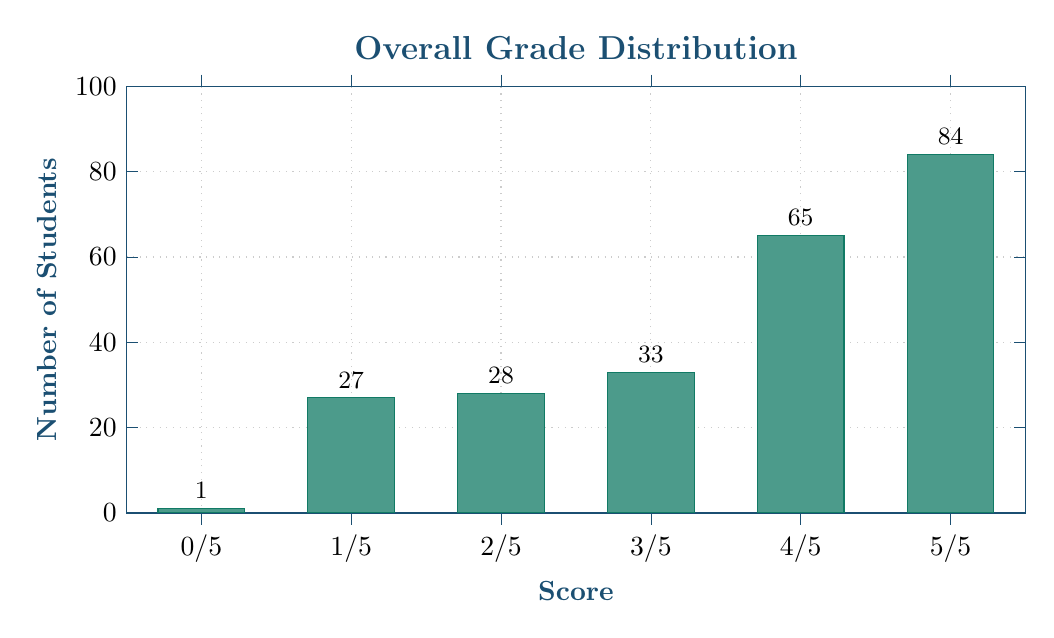
\begin{tikzpicture}
			\begin{axis}[
				ybar,
				width=13cm, height=7cm,
				bar width=1.1cm,
				xlabel={\textbf{Score}},
				ylabel={\textbf{Number of Students}},
				xtick={0,1,2,3,4,5},
				xticklabels={0/5, 1/5, 2/5, 3/5, 4/5, 5/5},
				ymin=0, ymax=100,
				nodes near coords,
				nodes near coords align={vertical},
				every node near coord/.style={font=\small\bfseries},
				grid=major,
				grid style={dotted, gray!40},
				axis line style={color=primary},
				tick style={color=primary},
				label style={color=primary},
				title={\textbf{\color{primary}Overall Grade Distribution}},
				title style={font=\large},
				]
				\addplot[fill=accent!75, draw=accent] coordinates {
					(0,1) (1,27) (2,28) (3,33) (4,65) (5,84)
				};
			\end{axis}
		\end{tikzpicture}
		\caption{Score distribution across all 238 students}
	\end{figure}
	
	% ─────────────────────────────────────────────────────────────────────────────
	\section{Per-Version Statistics}
	
	\begin{table}[H]
		\centering
		\caption{Descriptive statistics broken down by exam version}
		\renewcommand{\arraystretch}{1.35}
		\begin{tabular}{
				>{\centering\arraybackslash}m{1.2cm}
				>{\centering\arraybackslash}m{0.9cm}
				>{\centering\arraybackslash}m{1.4cm}
				>{\centering\arraybackslash}m{1.4cm}
				>{\centering\arraybackslash}m{1.4cm}
				>{\centering\arraybackslash}m{1.4cm}
				>{\centering\arraybackslash}m{0.9cm}
				>{\centering\arraybackslash}m{0.9cm}
			}
			\toprule
			\rowcolor{primary}
			\color{white}\textbf{Version} &
			\color{white}\textbf{N} &
			\color{white}\textbf{Mean} &
			\color{white}\textbf{\%} &
			\color{white}\textbf{Median} &
			\color{white}\textbf{Std Dev} &
			\color{white}\textbf{Min} &
			\color{white}\textbf{Max} \\
			\midrule
			\rowcolor{rowA} A & 19 & 3.947 & 78.9\% & 4.0 & 1.079 & 2 & 5 \\
			\rowcolor{rowB} B & 18 & 3.222 & 64.4\% & 3.0 & 1.114 & 2 & 5 \\
			\rowcolor{rowA} C & 26 & 4.077 & 81.5\% & 4.0 & 1.093 & 2 & 5 \\
			\rowcolor{rowB} D & 26 & 4.115 & 82.3\% & 5.0 & 1.366 & 0 & 5 \\
			\rowcolor{rowA} E & 26 & 4.000 & 80.0\% & 4.0 & 1.166 & 1 & 5 \\
			\rowcolor{rowB} F & 30 & 3.700 & 74.0\% & 4.0 & 1.368 & 1 & 5 \\
			\rowcolor{rowA} G & 15 & 3.000 & 60.0\% & 3.0 & 1.069 & 1 & 4 \\
			\rowcolor{success!15}
			H & 17 & \textbf{4.353} & \textbf{87.1\%} & 5.0 & 1.115 & 1 & 5 \\
			\rowcolor{danger!10}
			I & 29 & \textbf{2.517} & \textbf{50.3\%} & 3.0 & 1.243 & 1 & 4 \\
			\rowcolor{rowB} J & 32 & 3.406 & 68.1\% & 4.0 & 1.757 & 1 & 5 \\
			\bottomrule
		\end{tabular}
	\end{table}
	
	% ─── Version Mean Bar Chart ───────────────────────────────────────────────────
	\begin{figure}[H]
		\centering
		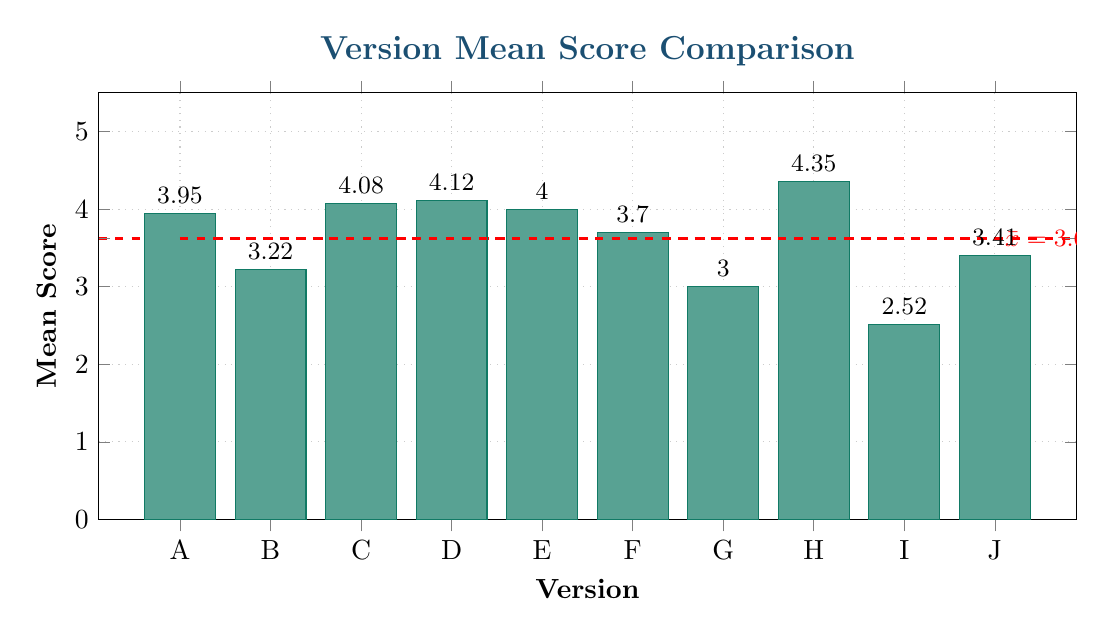
\begin{tikzpicture}
			\begin{axis}[
				ybar,
				width=14cm, height=7cm,
				bar width=0.9cm,
				symbolic x coords={A,B,C,D,E,F,G,H,I,J},
				xtick=data,
				xlabel={\textbf{Version}},
				ylabel={\textbf{Mean Score}},
				ymin=0, ymax=5.5,
				nodes near coords,
				nodes near coords style={font=\small\bfseries},
				grid=major,
				grid style={dotted, gray!40},
				title={\textbf{\color{primary}Version Mean Score Comparison}},
				title style={font=\large},
				extra y ticks={3.622},
				extra y tick labels={},
				extra y tick style={
					grid=major,
					grid style={dashed, red, thick}
				},
				]
				\addplot[fill=accent!70, draw=accent] coordinates {
					(A,3.947)(B,3.222)(C,4.077)(D,4.115)(E,4.0)
					(F,3.7)(G,3.0)(H,4.353)(I,2.517)(J,3.406)
				};
				\draw[red, dashed, thick] (axis cs:A,3.622) -- (axis cs:J,3.622)
				node[right, font=\small\color{red}] {$\bar{x}=3.622$};
			\end{axis}
		\end{tikzpicture}
		\caption{Mean score per version. Red dashed line = overall mean (3.622).}
	\end{figure}
	
	% ─────────────────────────────────────────────────────────────────────────────
	\section{Answer Choice Analysis by Question}
	
	\begin{table}[H]
		\centering
		\caption{Answer choice distribution across all students}
		\renewcommand{\arraystretch}{1.35}
		\begin{tabular}{
				>{\centering\bfseries\arraybackslash}m{1.2cm}
				>{\centering\arraybackslash}m{2.8cm}
				>{\centering\arraybackslash}m{2.8cm}
				>{\centering\arraybackslash}m{2.8cm}
				>{\centering\arraybackslash}m{2.8cm}
				>{\centering\arraybackslash}m{2cm}
			}
			\toprule
			\rowcolor{primary}
			\color{white}\textbf{Q} &
			\color{white}\textbf{A} &
			\color{white}\textbf{B} &
			\color{white}\textbf{C} &
			\color{white}\textbf{D} &
			\color{white}\textbf{Blank} \\
			\midrule
			\rowcolor{rowA} Q1 & 65 (27.3\%) & 124 (52.1\%) & 31 (13.0\%) & 18 (7.6\%)  & -- \\
			\rowcolor{rowB} Q2 & 50 (21.0\%) & 141 (59.2\%) & 20 (8.4\%)  & 27 (11.3\%) & -- \\
			\rowcolor{rowA} Q3 & 35 (14.7\%) & 97 (40.8\%)  & 91 (38.2\%) & 15 (6.3\%)  & -- \\
			\rowcolor{rowB} Q4 & 52 (21.8\%) & 114 (47.9\%) & 64 (26.9\%) & 8 (3.4\%)   & -- \\
			\rowcolor{rowA} Q5 & 65 (27.3\%) & 86 (36.1\%)  & 39 (16.4\%) & 47 (19.7\%) & 1 (0.4\%) \\
			\bottomrule
		\end{tabular}
	\end{table}
	
	% ─────────────────────────────────────────────────────────────────────────────
	\newpage
	\section{Answer Choice Analysis by Version}
	
	\subsection{Question 1}
	
	\begin{table}[H]
		\centering
		\renewcommand{\arraystretch}{1.3}
		\begin{tabular}{ccccc}
			\toprule
			\rowcolor{primary}
			\color{white}\textbf{Version} &
			\color{white}\textbf{A} &
			\color{white}\textbf{B} &
			\color{white}\textbf{C} &
			\color{white}\textbf{D} \\
			\midrule
			\rowcolor{rowA} A & 16\% & 58\% & 16\% & 11\% \\
			\rowcolor{rowB} B & 72\% & 17\% &  0\% & 11\% \\
			\rowcolor{rowA} C &  0\% & 85\% &  8\% &  8\% \\
			\rowcolor{rowB} D & 77\% & 15\% &  4\% &  4\% \\
			\rowcolor{rowA} E & 15\% &  0\% & 81\% &  4\% \\
			\rowcolor{rowB} F & 10\% & 80\% &  3\% &  7\% \\
			\rowcolor{rowA} G & 87\% &  7\% &  0\% &  7\% \\
			\rowcolor{rowB} H & 18\% & 71\% &  6\% &  6\% \\
			\rowcolor{rowA} I & 10\% & 83\% &  7\% &  0\% \\
			\rowcolor{rowB} J &  9\% & 72\% &  0\% & 19\% \\
			\bottomrule
		\end{tabular}
	\end{table}
	
	\subsection{Question 2}
	
	\begin{table}[H]
		\centering
		\renewcommand{\arraystretch}{1.3}
		\begin{tabular}{ccccc}
			\toprule
			\rowcolor{primary}
			\color{white}\textbf{Version} &
			\color{white}\textbf{A} &
			\color{white}\textbf{B} &
			\color{white}\textbf{C} &
			\color{white}\textbf{D} \\
			\midrule
			\rowcolor{rowA} A & 11\% & 84\% &  0\% &  5\% \\
			\rowcolor{rowB} B &  6\% & 94\% &  0\% &  0\% \\
			\rowcolor{rowA} C &  0\% & 85\% &  0\% & 15\% \\
			\rowcolor{rowB} D &  8\% &  0\% &  8\% & 85\% \\
			\rowcolor{rowA} E &  0\% & 96\% &  4\% &  0\% \\
			\rowcolor{rowB} F & 63\% & 13\% & 23\% &  0\% \\
			\rowcolor{rowA} G & 13\% & 87\% &  0\% &  0\% \\
			\rowcolor{rowB} H & 94\% &  6\% &  0\% &  0\% \\
			\rowcolor{rowA} I & 17\% & 55\% & 28\% &  0\% \\
			\rowcolor{rowB} J &  9\% & 84\% &  6\% &  0\% \\
			\bottomrule
		\end{tabular}
	\end{table}
	
	\subsection{Question 3}
	
	\begin{table}[H]
		\centering
		\renewcommand{\arraystretch}{1.3}
		\begin{tabular}{ccccc}
			\toprule
			\rowcolor{primary}
			\color{white}\textbf{Version} &
			\color{white}\textbf{A} &
			\color{white}\textbf{B} &
			\color{white}\textbf{C} &
			\color{white}\textbf{D} \\
			\midrule
			\rowcolor{rowA} A & 11\% & 11\% & 79\% &  0\% \\
			\rowcolor{rowB} B & 11\% & 83\% &  6\% &  0\% \\
			\rowcolor{rowA} C &  4\% & 85\% &  4\% &  8\% \\
			\rowcolor{rowB} D &  0\% & 85\% & 12\% &  4\% \\
			\rowcolor{rowA} E &  8\% &  8\% & 81\% &  4\% \\
			\rowcolor{rowB} F & 10\% & 10\% & 70\% & 10\% \\
			\rowcolor{rowA} G & 87\% & 13\% &  0\% &  0\% \\
			\rowcolor{rowB} H &  0\% &100\% &  0\% &  0\% \\
			\rowcolor{rowA} I & 24\% & 28\% & 24\% & 24\% \\
			\rowcolor{rowB} J & 16\% & 12\% & 69\% &  3\% \\
			\bottomrule
		\end{tabular}
	\end{table}
	
	\subsection{Question 4}
	
	\begin{table}[H]
		\centering
		\renewcommand{\arraystretch}{1.3}
		\begin{tabular}{ccccc}
			\toprule
			\rowcolor{primary}
			\color{white}\textbf{Version} &
			\color{white}\textbf{A} &
			\color{white}\textbf{B} &
			\color{white}\textbf{C} &
			\color{white}\textbf{D} \\
			\midrule
			\rowcolor{rowA} A & 95\% &  5\% &  0\% &  0\% \\
			\rowcolor{rowB} B &  0\% & 78\% & 17\% &  6\% \\
			\rowcolor{rowA} C &  4\% &  0\% & 96\% &  0\% \\
			\rowcolor{rowB} D &  4\% & 85\% & 12\% &  0\% \\
			\rowcolor{rowA} E &  8\% & 85\% &  0\% &  8\% \\
			\rowcolor{rowB} F &  3\% & 93\% &  3\% &  0\% \\
			\rowcolor{rowA} G & 87\% &  0\% & 13\% &  0\% \\
			\rowcolor{rowB} H &  0\% &  6\% & 94\% &  0\% \\
			\rowcolor{rowA} I & 45\% & 31\% & 14\% & 10\% \\
			\rowcolor{rowB} J &  9\% & 53\% & 31\% &  6\% \\
			\bottomrule
		\end{tabular}
	\end{table}
	
	\subsection{Question 5}
	
	\begin{table}[H]
		\centering
		\renewcommand{\arraystretch}{1.3}
		\begin{tabular}{ccccc}
			\toprule
			\rowcolor{primary}
			\color{white}\textbf{Version} &
			\color{white}\textbf{A} &
			\color{white}\textbf{B} &
			\color{white}\textbf{C} &
			\color{white}\textbf{D} \\
			\midrule
			\rowcolor{rowA} A & 11\% & 79\% &  5\% &  5\% \\
			\rowcolor{rowB} B & 17\% & 17\% & 17\% & 50\% \\
			\rowcolor{rowA} C & 35\% & 58\% &  8\% &  0\% \\
			\rowcolor{rowB} D & 15\% & 81\% &  4\% &  0\% \\
			\rowcolor{rowA} E &  8\% & 31\% &  4\% & 58\% \\
			\rowcolor{rowB} F & 33\% &  0\% & 63\% &  3\% \\
			\rowcolor{rowA} G & 20\% & 40\% &  7\% & 33\% \\
			\rowcolor{rowB} H &  0\% & 12\% & 12\% & 76\% \\
			\rowcolor{rowA} I & 41\% & 52\% &  0\% &  7\% \\
			\rowcolor{rowB} J & 62\% &  3\% & 28\% &  3\% \\
			\bottomrule
		\end{tabular}
	\end{table}
	
	% ─────────────────────────────────────────────────────────────────────────────
	\section{Version Comparison — Difficulty Ranking}
	
	\begin{table}[H]
		\centering
		\caption{Versions ranked from easiest to hardest by mean score}
		\renewcommand{\arraystretch}{1.4}
		\begin{tabular}{
				>{\centering\arraybackslash}m{1cm}
				>{\centering\arraybackslash}m{1.5cm}
				>{\centering\arraybackslash}m{2cm}
				>{\centering\arraybackslash}m{3cm}
			}
			\toprule
			\rowcolor{primary}
			\color{white}\textbf{Rank} &
			\color{white}\textbf{Version} &
			\color{white}\textbf{Mean} &
			\color{white}\textbf{Difficulty} \\
			\midrule
			\rowcolor{success!20} 1 & H & 4.353 & \textcolor{success}{\textbf{Easy}} \\
			\rowcolor{success!15} 2 & D & 4.115 & \textcolor{success}{\textbf{Easy}} \\
			\rowcolor{success!10} 3 & C & 4.077 & \textcolor{success}{\textbf{Easy}} \\
			\rowcolor{success!10} 4 & E & 4.000 & \textcolor{success}{\textbf{Easy}} \\
			\rowcolor{success!5}  5 & A & 3.947 & \textcolor{success}{\textbf{Easy}} \\
			\rowcolor{warning!15} 6 & F & 3.700 & \textcolor{warning!80!black}{\textbf{Moderate}} \\
			\rowcolor{warning!15} 7 & J & 3.406 & \textcolor{warning!80!black}{\textbf{Moderate}} \\
			\rowcolor{warning!10} 8 & B & 3.222 & \textcolor{warning!80!black}{\textbf{Moderate}} \\
			\rowcolor{warning!10} 9 & G & 3.000 & \textcolor{warning!80!black}{\textbf{Moderate}} \\
			\rowcolor{danger!15} 10 & I & 2.517 & \textcolor{danger}{\textbf{Hard}} \\
			\bottomrule
		\end{tabular}
	\end{table}
	
	% ─── Statistical Tests ────────────────────────────────────────────────────────
	\subsection{Statistical Equivalence Tests}
	
	\begin{table}[H]
		\centering
		\caption{ANOVA and Kruskal-Wallis tests for version equivalence}
		\renewcommand{\arraystretch}{1.4}
		\begin{tabular}{lccc}
			\toprule
			\rowcolor{primary}
			\color{white}\textbf{Test} &
			\color{white}\textbf{Statistic} &
			\color{white}\textbf{p-value} &
			\color{white}\textbf{Result} \\
			\midrule
			\rowcolor{rowA} ANOVA (parametric)        & $F = 4.7962$ & $7 \times 10^{-6}$ &
			\textcolor{danger}{\textbf{$\times$ Significant difference}} \\
			\rowcolor{rowB} Kruskal-Wallis (non-param) & $H = 42.6413$ & $3 \times 10^{-6}$ &
			\textcolor{danger}{\textbf{$\times$ Significant difference}} \\
			\bottomrule
		\end{tabular}
	\end{table}
	
	\begin{tcolorbox}[colback=danger!5, colframe=danger, arc=3pt, boxrule=0.8pt]
		\textbf{Interpretation:} Both tests confirm that exam versions are \textbf{NOT statistically
			equivalent} ($p \ll 0.05$). This suggests that students received unfairly different levels
		of difficulty depending on their assigned version.
	\end{tcolorbox}
	
	\subsection{Outlier Versions (Z-Score Analysis)}
	
	\begin{table}[H]
		\centering
		\caption{Z-scores relative to grand mean (3.634) and std dev (0.582)}
		\renewcommand{\arraystretch}{1.4}
		\begin{tabular}{cccc}
			\toprule
			\rowcolor{primary}
			\color{white}\textbf{Version} &
			\color{white}\textbf{Mean} &
			\color{white}\textbf{Z-Score} &
			\color{white}\textbf{Note} \\
			\midrule
			\rowcolor{rowA}          A & 3.947 & $+0.54$ & \\
			\rowcolor{rowB}          B & 3.222 & $-0.71$ & \\
			\rowcolor{rowA}          C & 4.077 & $+0.76$ & \\
			\rowcolor{rowB}          D & 4.115 & $+0.83$ & \\
			\rowcolor{rowA}          E & 4.000 & $+0.63$ & \\
			\rowcolor{rowB}          F & 3.700 & $+0.11$ & \\
			\rowcolor{warning!20}    G & 3.000 & $-1.09$ &
			\textcolor{warning!80!black}{\textbf{$\leftarrow$ Significantly HARDER}} \\
			\rowcolor{success!15}    H & 4.353 & $+1.24$ &
			\textcolor{success}{\textbf{$\leftarrow$ Significantly EASIER}} \\
			\rowcolor{danger!15}     I & 2.517 & $-1.92$ &
			\textcolor{danger}{\textbf{$\leftarrow$ Significantly HARDER}} \\
			\rowcolor{rowB}          J & 3.406 & $-0.39$ & \\
			\bottomrule
		\end{tabular}
	\end{table}
	
	% ─────────────────────────────────────────────────────────────────────────────
	\section{Quick Summary}
	
	\begin{summarybox}
		\begin{itemize}[leftmargin=*, itemsep=4pt]
			\item \textbf{Total Students:} 238
			\item \textbf{Overall Mean:} 3.622 / 5 \quad (72.4\%)
			\item \textbf{Overall Median:} 4.0
			\item \textbf{Overall Mode:} 5
			\item \textbf{Overall Std Dev:} 1.384
			\item \textbf{Easiest Version:} H \quad (mean = 4.353, 87.1\%)
			\item \textbf{Hardest Version:} I \quad (mean = 2.517, 50.3\%)
			\item \textbf{Spread in Means:} 1.836 points across versions
			\item \textbf{ANOVA p-value:} $7 \times 10^{-6}$ \quad
			\textcolor{danger}{$\rightarrow$ Versions are \textbf{NOT} statistically equivalent}
		\end{itemize}
	\end{summarybox}
	
	\vfill
	\begin{center}
		\textcolor{medgray}{\small\rule{0.4\textwidth}{0.4pt} \\[4pt]
			End of Report — Generated by Euler OMR Grading System}
	\end{center}
	
\end{document}